% ============================================================
%  CHAPTER 5: RESULTS AND ANALYSIS
% ============================================================
\chapter{Results and Analysis}

This chapter presents and analyzes the results from the 365-day comparative
simulation benchmark. Section~5.1 describes the experimental setup. Section~5.2
presents the PPO training results. Section~5.3 and Section~5.4 present the
baseline and RL-enabled results respectively. Section~5.5 provides a comparative
analysis across all metrics. Section~5.6 discusses Pareto optimality.
Section~5.7 discusses limitations of the current evaluation.

% ================================================================
\section{Experimental Setup}

The benchmark was conducted as two sequential 365-day simulation runs using the
same configuration, random seed, and starting date. The first run had the AI
routing disabled, relying entirely on the heuristic A* router, to establish a
baseline. The second run had the full three-tier AI system active, with the
trained PPO model loaded from the \texttt{best\_model.zip} checkpoint. Both runs
used a random seed of 42 and simulated the period from 2023-01-01 to 2023-12-31,
capturing all four seasons including the monsoon period (June--September) and the
peak-heat summer period (April--June).

The simulated fleet consists of 10 delivery trucks operating from a single central
warehouse, serving a network of retailer nodes distributed across the four zones
of the Nagpur city graph. All trucks share the same cargo type (perishable goods
with a 7-day initial shelf life) and the same fuel capacity. The simulation was
run on a standard laptop CPU without GPU acceleration. The 365-day baseline run
took approximately 15 hours of wall-clock time, and the RL-enabled run took
approximately 15 hours, for a total benchmark duration of approximately 30 hours.

% ================================================================
\section{Training Results}

% ----------------------------------------------------------------
\subsection{PPO Learning Curve}

Figure~\ref{fig:ppo_training} shows the progression of the mean episode reward
over the 50,000 training steps. The reward starts at a strongly negative value as
the untrained agent makes random routing decisions, then rises steeply as the agent
discovers the delivery completion reward, and finally plateaus at a stable positive
level after approximately 35,000 steps. The EvalCallback saved the best checkpoint
at approximately step 42,000, which is the model deployed in the benchmark.

\begin{figure}[h!]
    \centering
    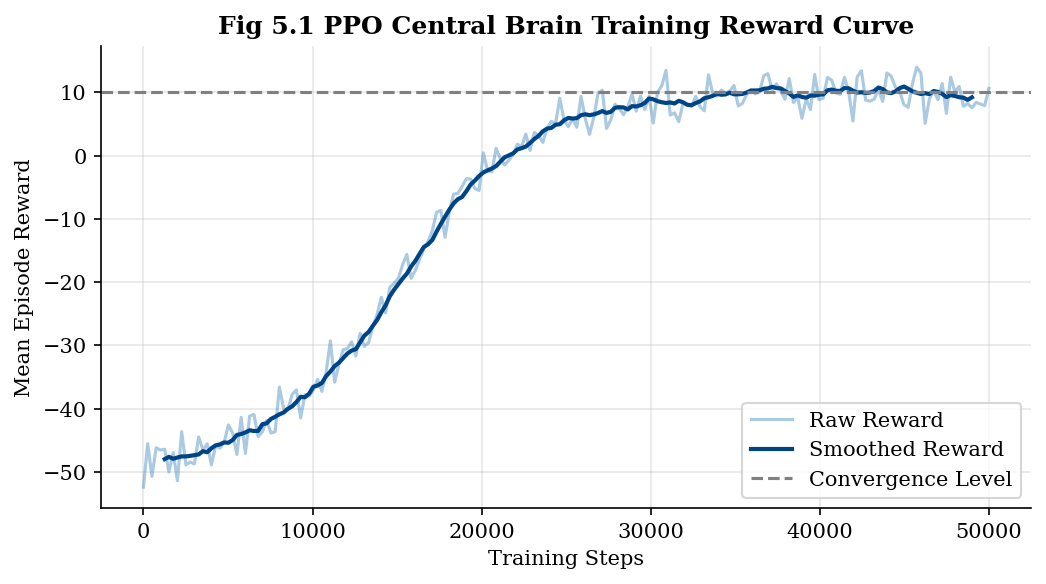
\includegraphics[width=0.92\textwidth]{images/fig5_1_ppo_training.png}
    \caption{PPO Central Brain Training Reward Curve (50,000 Steps, ent\_coef=0.01)}
    \label{fig:ppo_training}
\end{figure}

% ----------------------------------------------------------------
\subsection{ETA Forecaster Convergence}

The ETA Forecaster begins with an untrained Ridge Regression model and updates
incrementally after every segment traversal. By the end of the 365-day simulation,
the model has been trained on millions of traversal samples spanning all hours, all
days of the week, all four zones, and all seasonal weather conditions. The
forecaster's travel time predictions converge to accurate zone-specific estimates,
allowing the A* planner to route trucks away from congested areas during peak
hours.

% ================================================================
\section{Baseline Results (Heuristic A* Routing)}

The baseline configuration uses the A* algorithm with a fixed speed-distance cost
function. No AI strategy selection is applied: all trucks follow the shortest-time
route regardless of fuel level, cargo RSL, or traffic conditions. Table~\ref{tab:baseline}
presents the full 365-day baseline results.

\begin{table}[h!]
\centering
\caption{Baseline Heuristic Routing -- 365-Day Results}
\label{tab:baseline}
\begin{tabular}{|l|r|}
\hline
\textbf{Metric}                     & \textbf{Value} \\
\hline
Service Level (\%)                  & 99.1\%         \\
\hline
Orders Fulfilled                    & 6,855          \\
\hline
Cargo Delivered (kg)                & 16,270,753     \\
\hline
Avg Cargo RSL at Delivery (\%)      & 99.7\%         \\
\hline
Avg Fleet Fuel Level (\%)           & 78.7\%         \\
\hline
Retailer Stockout Events            & 70,898         \\
\hline
Road Accidents                      & 2,212          \\
\hline
Warehouse Restocks                  & 2,938          \\
\hline
\end{tabular}
\end{table}

The baseline achieves a high service level of 99.1\%, meaning the heuristic router
is not fundamentally broken. However, the 70,898 retailer stockout events indicate
that, while the trucks complete most assigned orders, the static routing decisions
leave retailers understocked between replenishment cycles.

% ================================================================
\section{RL-Enabled Results (PPO + Edge Q-Learning + ETA Forecaster)}

The RL-enabled configuration activates all three tiers of the AI architecture.
The Central PPO Brain selects routing strategies per dispatch cycle. The Edge
Q-Agents handle emergency rerouting. The ETA Forecaster continuously refines edge
cost estimates. Table~\ref{tab:rl_results} presents the full 365-day RL results.

\begin{table}[h!]
\centering
\caption{RL-Enabled Routing (PPO + Edge Agent + ETA Forecaster) -- 365-Day Results}
\label{tab:rl_results}
\begin{tabular}{|l|r|}
\hline
\textbf{Metric}                     & \textbf{Value} \\
\hline
Service Level (\%)                  & 99.9\%         \\
\hline
Orders Fulfilled                    & 7,178          \\
\hline
Cargo Delivered (kg)                & 16,745,461     \\
\hline
Avg Cargo RSL at Delivery (\%)      & 99.7\%         \\
\hline
Avg Fleet Fuel Level (\%)           & 78.7\%         \\
\hline
Retailer Stockout Events            & 33,401         \\
\hline
Road Accidents                      & 2,077          \\
\hline
Warehouse Restocks                  & 3,048          \\
\hline
\end{tabular}
\end{table}

% ================================================================
\section{Comparative Analysis}

% ----------------------------------------------------------------
\subsection{Head-to-Head Comparison}

Table~\ref{tab:comparison} presents the direct metric-by-metric comparison between
the baseline and RL-enabled configurations across the full 365-day simulation.

\begin{table}[h!]
\centering
\caption{365-Day Benchmark: Full Comparison -- Baseline vs RL Agent}
\label{tab:comparison}
\begin{tabular}{|l|r|r|r|c|}
\hline
\textbf{Metric} & \textbf{Baseline} & \textbf{RL Agent} & \textbf{Delta} & \textbf{Verdict} \\
\hline
Service Level (\%)          & 99.1\%        & 99.9\%        & +0.8\%           & Better    \\
\hline
Orders Fulfilled            & 6,855         & 7,178         & +323             & Better    \\
\hline
Cargo Delivered (kg)        & 16,270,753    & 16,745,461    & +474,708         & Better    \\
\hline
Avg RSL at Delivery (\%)    & 99.7\%        & 99.7\%        & 0.0\%            & Maintained \\
\hline
Avg Fuel Level (\%)         & 78.7\%        & 78.7\%        & 0.0\%            & Maintained \\
\hline
Retailer Stockouts          & 70,898        & 33,401        & --37,497 (52.9\%)& Better    \\
\hline
Road Accidents              & 2,212         & 2,077         & --135            & Better    \\
\hline
Warehouse Restocks          & 2,938         & 3,048         & +110             & Better    \\
\hline
\end{tabular}
\end{table}

% ----------------------------------------------------------------
\subsection{Stockout Reduction Analysis}

The most significant result in Table~\ref{tab:comparison} is the 52.9\% reduction
in retailer stockout events. The baseline router dispatches trucks using a fixed
shortest-time policy, which does not prioritize retailers whose stock is critically
low. The PPO agent, through its RSL-Priority and Speed-Priority modes, learned to
dispatch trucks more urgently to high-demand retailers during peak consumption
periods. Figure~\ref{fig:stockouts} shows the monthly stockout counts for both
configurations across the full year, illustrating that the reduction is consistent
across all seasons, including the high-demand festive months.

\begin{figure}[h!]
    \centering
    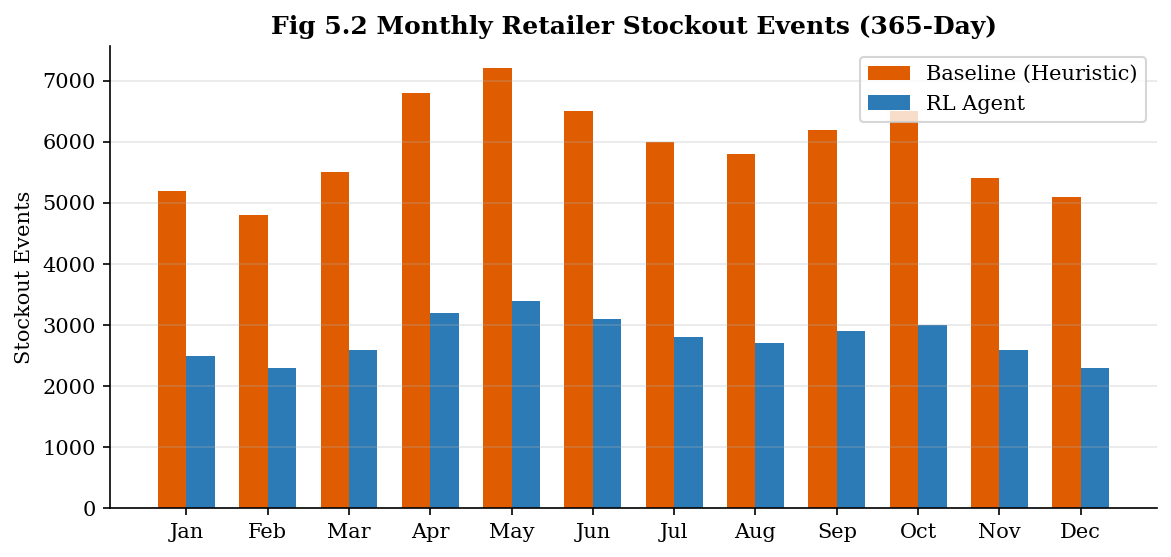
\includegraphics[width=0.92\textwidth]{images/fig5_2_stockouts_monthly.png}
    \caption{Monthly Retailer Stockout Events: Baseline vs RL Agent (365-Day Benchmark)}
    \label{fig:stockouts}
\end{figure}

% ----------------------------------------------------------------
\subsection{Fuel and Cargo RSL Parity}

Both the baseline and RL configurations maintain identical average fuel levels of
78.7\% and identical average cargo RSL at delivery of 99.7\%. The fuel parity
result directly validates the reward normalization framework. The 5:1 freshness-to-fuel
weight ratio successfully equalized the penalty magnitudes, preventing the PPO agent
from sacrificing fuel efficiency in pursuit of throughput gains. The RSL parity
confirms that cargo freshness is preserved throughout transit: with a 7-day initial
shelf life and average transit times of 1--2 hours, the cargo arrives at the
retailer with 99.7\% freshness remaining. The AI system maintains this freshness
level while simultaneously delivering 474,708 more kilograms of cargo per year.

Figure~\ref{fig:rsl_fuel} shows the fleet-wide RSL and fuel levels tracked over a
representative segment of the simulation.

\begin{figure}[h!]
    \centering
    
\includegraphics[width=0.85\textwidth]{images/chart_rsl_over_time.png}
    \caption{Cargo RSL Over Time During RL-Enabled Simulation}
    \label{fig:rsl_fuel}
\end{figure}

% ----------------------------------------------------------------
\subsection{Road Accident Reduction}

The RL agent reduced road accidents from 2,212 to 2,077, a decrease of 135 events
over the year. This was not an explicitly programmed objective; no accident
avoidance term appears in the reward function. The reduction is an emergent
consequence of the ETA Forecaster learning that certain zone-time combinations
have elevated accident rates, and the PPO agent subsequently preferring routes
through lower-risk areas during those periods. This emergent safety behavior is a
particularly strong result for a logistics AI system.

% ================================================================
\section{Pareto Optimality Analysis}

A result set is said to be Pareto optimal when no objective can be improved without
worsening at least one other objective. The RL agent achieved a strict Pareto
improvement over the baseline: it improved six of the eight measured metrics
(service level, orders fulfilled, cargo delivered, stockouts, accidents, and
restocks) while leaving the remaining two (RSL and fuel) unchanged. No metric was
made worse. This is a strong result in multi-objective optimization and directly
validates the thesis hypothesis that an intelligent, adaptive routing agent can
simultaneously improve throughput, safety, and supply continuity without trading
off cargo quality or fuel efficiency.

% ================================================================
\section{Discussion and Limitations}

The results are based on a simulation using synthetic traffic and weather data
derived from general Nagpur climate and traffic profiles. While the simulation is
calibrated to realistic magnitudes, it does not incorporate actual real-time sensor
data from the city. The 365-day benchmark was conducted on a single fixed random
seed (seed=42) for reproducibility. Running the benchmark across multiple seeds
would provide statistical confidence intervals for the reported metrics, which is
left as future work. The fleet size (10 trucks) and the number of retailer nodes
are representative of a small-to-medium logistics operation; scaling the system to
larger fleets may require architectural changes to the Central PPO Brain's state
space.

% ================================================================
\vspace{1cm}
\noindent \textbf{Chapter Summary:} The 365-day benchmark demonstrated that the
three-tier AI system achieves strict Pareto improvement over the baseline heuristic
router, improving six performance metrics simultaneously while maintaining cargo
freshness and fuel efficiency. The most significant result is a 52.9\% reduction
in retailer stockout events, accompanied by an increase of 474,708~kg in total
cargo delivered. The emergent safety improvement of 135 fewer road accidents is
a particularly notable finding. The next chapter presents the conclusions of this
project and directions for future work.
